\section{Defects}
\label{sec:defects}

The defect rung of \S\ref{sec:object} is short to state and expensive to
draw by hand. A circle-valued field, encoded at integer gain, ends
fringes. The signed count of those endings is the enclosed charge times
the gain: quantized, localized, additive, and blind to any exact field
added on top. This section is that statement, drawn.

Everything so far took $f$ single-valued, and one spelling in the language
quietly is not. \texttt{theta} is a branch of the polar angle, well defined
only modulo full turns, so \texttt{theta\,/\,tau} is a \emph{circle-valued}
field: defined modulo $1$ on the punctured plane, gaining one unit per
positive loop around the origin. Encoded at an integer gain $a=A$, the index
difference $D=A\,\theta/\tau$ is multivalued, but its fringe set
$\{D\in\Z\}$ is perfectly well defined, and it is a pencil of $A$ rays. A
fringe now does something no single-valued field permits: it \emph{ends}.
Along any loop $\gamma$ avoiding the singularities of $f$, the signed count
of fringe crossings is the degree of the circle-valued map $D\circ\gamma$,
which is $A$ times the total winding of $f$ enclosed; level sets cannot
terminate where $D$ is regular, so the signed number of fringe endings inside
$\gamma$ equals the enclosed charge times the gain. We
verified each clause by counting integer crossings on probe loops
(\texttt{tools\pslash exp\pslash defects.mjs}): $\defProbes$ probes spanning
gains $1$ to $\defChargeMax$, displaced defects, opposite-charge pairs, and a
defect plus an exact field, every count exact.

\begin{figure*}[t]
  \centering
  \begin{subfigure}{0.325\textwidth}
    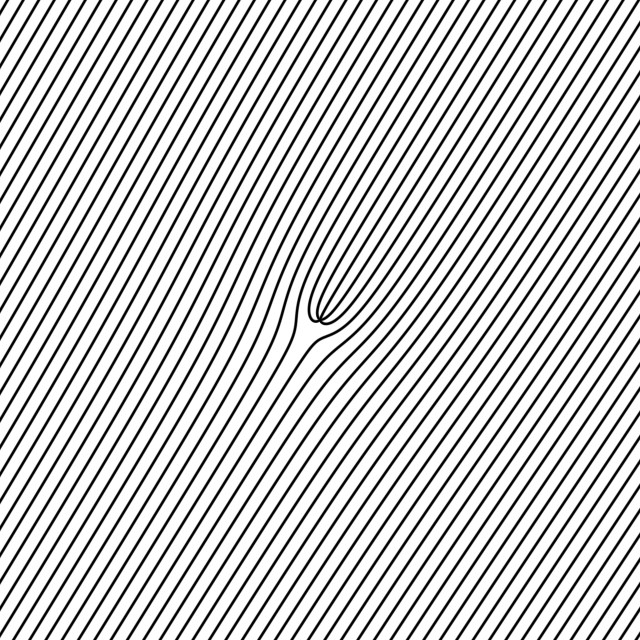
\includegraphics[width=\linewidth]{figures/defect-fork.png}
    \caption{one family, $f=\theta/\tau$, $a=5$}
  \end{subfigure}\hfill
  \begin{subfigure}{0.325\textwidth}
    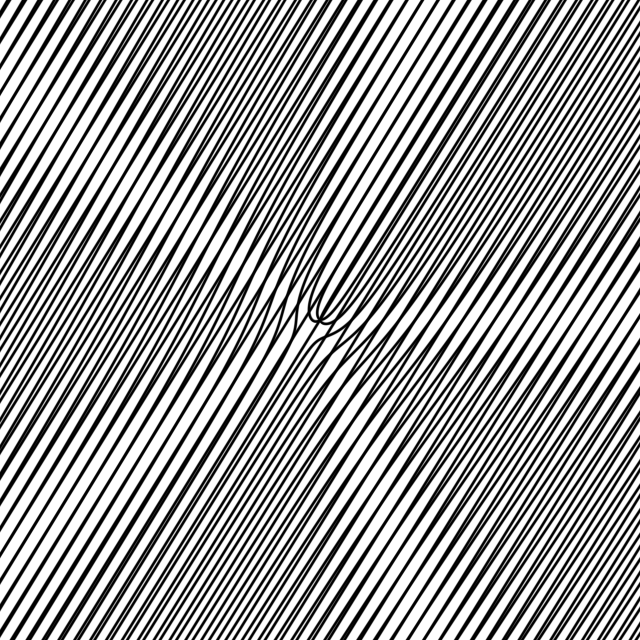
\includegraphics[width=\linewidth]{figures/defect-pair.png}
    \caption{over its unmodulated twin}
  \end{subfigure}\hfill
  \begin{subfigure}{0.325\textwidth}
    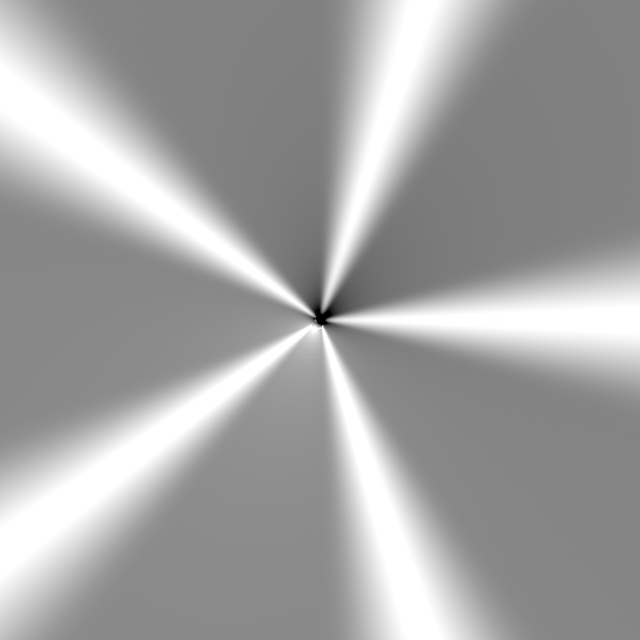
\includegraphics[width=\linewidth]{figures/defect-envelope.png}
    \caption{envelope: five fringes end}
  \end{subfigure}
  \Description{Three square panels. The first is a field of fine diagonal lines
  in which five extra lines fan out of a point at the center, like a fork with
  five tines. The second overlays that family on a plain copy of itself,
  producing a subtle pinwheel of light and dark around the same point. The
  third is the smooth averaged view: five bright wedge-shaped fringes radiate
  from the center and stop there, with a small dark core at the very middle.}
  \caption{\figlead{A circle-valued field mints a defect.} \textbf{(a)}~A line
  family carrying $f=\theta/\tau$ at gain $5$ is the classical fork grating:
  five extra members emanate from the origin, where the family's counting
  fails to close. \textbf{(b)}~Against an unmodulated twin the moir\'e carries
  the defect. \textbf{(c)}~The envelope view: five fringes \emph{end} at the
  origin, the picture no single-valued field can draw, and the signed count
  of endings is exactly the winding times the gain. The dark spot is the
  defect core $r^\star=2As/\pi$, where $\het$ crosses $1/4$ and the fringe
  law honestly fails.}
  \label{fig:defects}
\end{figure*}

Figure~\ref{fig:defects} draws the smallest interesting case. A carrier plus
$A\,\theta/\tau$ is the \emph{fork grating}: $A$ extra members fan out of the
origin, which is how holography prints screw-dislocated
wavefronts~\cite{Bazhenov1990Screw}, and the fringe that ends is the edge
dislocation of Nye and Berry's wave-train
taxonomy~\cite{NyeBerry1974Dislocations, SoskinVasnetsov2001Singular}. In
singular optics these objects are measured; here they are \emph{authored},
typed into the field box at frame rate, and the radial pencil of
\S\ref{sec:catalog} is the same object one level down: its index
is $N\theta/\pi$, a pure winding field, so the pencil is the charge-$2N$
defect of the line family rather than an exception to the catalog.

The topology is exact but not free: near the defect the fringe spacing
$1/\lVert\nabla D\rVert = \tau r/A$ collapses, so the heterodyne ratio
against the twin is $\het = As/(\tau r)$, crossing the regime line
$1/4$ at the \emph{core radius} $r^\star = 2As/\pi$. We measured the crossing
against the evaluator's exact gradients and it lands on $r^\star$ to within
$\defCoreWorst$: inside the core the fringe law fails, the ratio view says so
(\S\ref{sec:visibility}), and the envelope's mask fades the region rather
than inventing fringes in it. The theory draws a circle around its own
failure. A \emph{non-integer} gain has no well-defined fringe set at all; the
tool renders the tear along the evaluator's branch cut, which carries the
fractional winding, an honest picture of an impossible request.
